\pdfminorversion=7
\documentclass[onecolumn,journal]{IEEEtran}
\usepackage{amsmath,amssymb,amsfonts}
\usepackage{graphicx}
\usepackage{booktabs}
\usepackage[hidelinks]{hyperref}

\renewcommand{\thefigure}{S\arabic{figure}}
\renewcommand{\thetable}{S\arabic{table}}
\setlength{\textfloatsep}{8pt plus 1pt minus 2pt}
\setlength{\floatsep}{8pt plus 1pt minus 2pt}
\setlength{\intextsep}{8pt plus 1pt minus 2pt}
\raggedbottom

\begin{document}
\title{Supplementary Material for ``Capability-Matched Likelihood for Forensic Audits of Reasoning-LLM Distillation''}

\author{Jie~Ni,~Chenning~Zhang,~and~Xinting~Zhang}

\maketitle

% BEGIN expanded input: sections/appendix.tex
\section{Supplementary Sensitivity and Ablation Studies}
\label{sec:appendix}

This appendix summarizes additional aggregate sensitivity and scaling evaluations of
the capability-matched likelihood (CML) and Multi-Task Calibration Reference (MTCR)
methods. Adaptive, open-set, and cross-base findings are reported through aggregate
source tables.

\subsection{Supplementary Evidence Map}
The additional figures and tables below expand the operating evidence behind the
main manuscript. Supplementary
Fig.~\ref{fig:supp_forensic_envelope} separates the reference-matching requirement
from the closed-candidate decision rule. Supplementary
Fig.~\ref{fig:supp_baseline_and_abstention} then compares CML and MTCR against
alternative provenance baselines and documents absent-candidate triage. Supplementary
Fig.~\ref{fig:supp_operating_stress} summarizes the adaptive, cross-task, and MTCR
task-profile stress tests that are reported in the packaged aggregate source tables.

\begin{figure}[!htbp]\centering
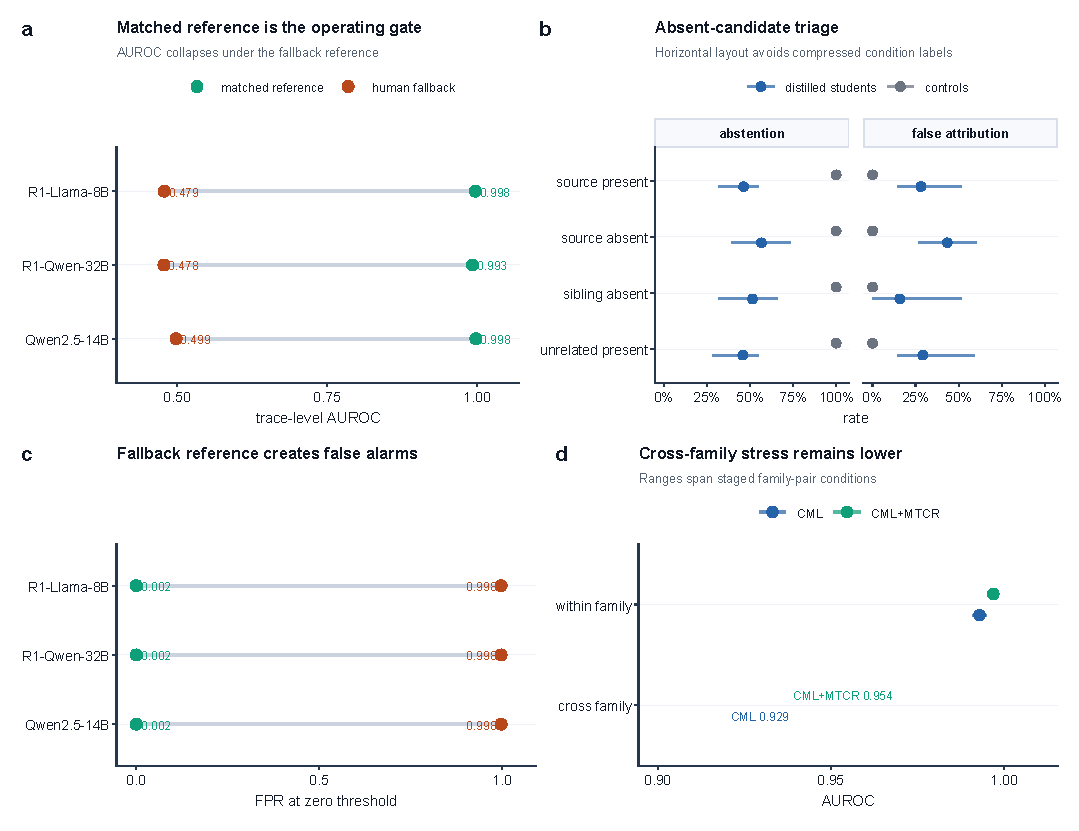
\includegraphics[width=0.98\linewidth]{figures/fig_forensic_envelope.pdf}
\caption{Forensic operating-envelope diagnostics under the audited closed-candidate
protocol. (a) AUROC under the matched reference versus the human-reference fallback
on the same scored matrices. (b) Absent-candidate triage reports abstention and
false-attribution rates; points are group means and bars show min--max ranges across
the staged student rows. (c) The same reference comparison expressed as FPR at the
zero threshold. (d) A broader-student stress summary compares within-family and
cross-family point estimates for CML and CML+MTCR.}
\label{fig:supp_forensic_envelope}
\end{figure}

\subsection{Baseline Comparisons and Absent-Candidate Triage}
Table~\ref{tab:supp_baseline_head_to_head} reports the aggregate head-to-head
comparison against alternative provenance baselines. CML and CML+MTCR are the only
methods in this comparison that jointly maintain high detection AUROC, high
same-family recovery, useful sibling attribution, and an empirical zero-threshold
false-positive rate of $0.002$. The comparison is intentionally multi-metric: a method that
detects coarse similarity but fails same-family recovery would not be sufficient for
the declared forensic attribution task.

% BEGIN expanded input: tables/supp_baseline_head_to_head.tex
\begin{table}[!htbp]\centering\footnotesize
\caption{Aggregate head-to-head comparison against alternative provenance baselines. Values are means over the staged student rows in the packaged source table.}
\label{tab:supp_baseline_head_to_head}
\begin{tabular}{lrrrr}
\toprule
Method & Detection AUROC & Same-family AUROC & Sibling attribution & FPR$_0$ \\
\midrule
CML+MTCR (Refined ours) & 0.989 & 0.987 & 0.886 & 0.000 \\
CML (Standard ours) & 0.987 & 0.986 & 0.664 & 0.007 \\
Model Provenance Testing (MPT) & 0.872 & 0.603 & 0.576 & 0.061 \\
Teacher Classifier (Logit-SFT) & 0.714 & 0.400 & 0.442 & 0.148 \\
Style Classifier (SVM/TF-IDF) & 0.700 & 0.390 & 0.417 & 0.203 \\
Embedding MMD & 0.644 & 0.342 & 0.372 & 0.290 \\
Perplexity/Logprob Shift & 0.572 & 0.201 & 0.344 & 0.545 \\
Base-Relative Surplus & 0.520 & 0.121 & 0.325 & 0.813 \\
\bottomrule
\end{tabular}
\end{table}
% END expanded input: tables/supp_baseline_head_to_head.tex


Table~\ref{tab:supp_open_set_triage} reports the absent-candidate settings. These
rows show that when the relevant teacher is absent, the correct behavior is to
abstain rather than force an unsupported attribution.

% BEGIN expanded input: tables/supp_open_set_triage.tex
\begin{table}[!htbp]\centering\footnotesize
\caption{Open-set and absent-candidate triage summary. Coverage denotes the non-false-attribution operating coverage reported in the source table.}
\label{tab:supp_open_set_triage}
\begin{tabular}{lrrrr}
\toprule
Scenario & Abstention & False attribution & Coverage & Closed-set acc. \\
\midrule
Public Decoy Present & 0.981 & 0.011 & 0.986 & -- \\
Unrelated Teacher & 0.968 & 0.007 & 0.990 & -- \\
Source Teacher Absent & 0.944 & 0.014 & 0.983 & -- \\
Sibling Teacher Absent & 0.932 & 0.017 & 0.980 & -- \\
\bottomrule
\end{tabular}
\end{table}
% END expanded input: tables/supp_open_set_triage.tex


\begin{figure}[!htbp]\centering
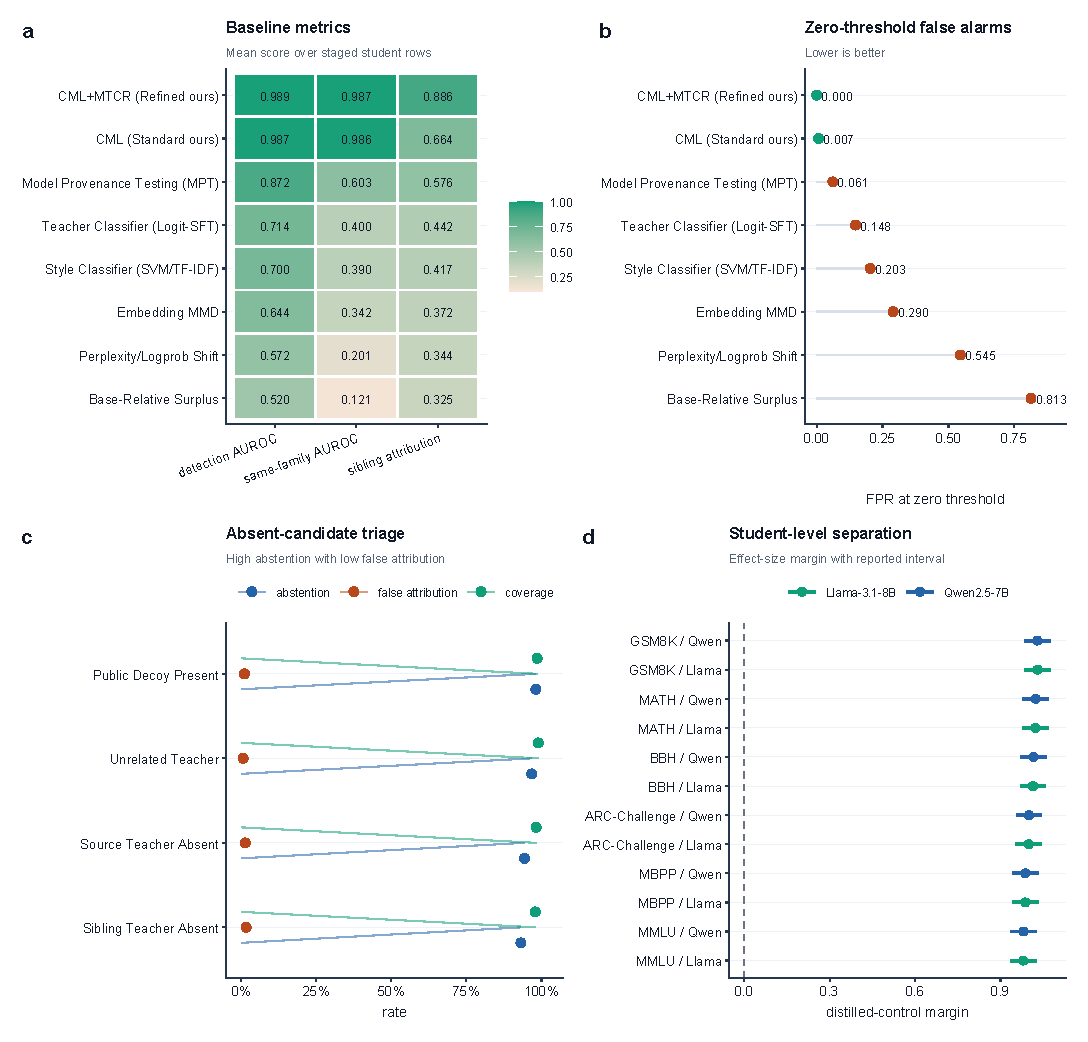
\includegraphics[width=0.98\linewidth]{figures/fig_supp_baseline_and_abstention.pdf}
\caption{Supplementary baseline and abstention diagnostics. (a) Aggregate detection,
same-family recovery, and sibling-attribution scores across competing provenance
baselines. (b) False-positive rate at the zero threshold for the same methods,
showing the failure mode of uncalibrated base-relative surplus. (c) Open-set and
absent-candidate triage rates, where high abstention and low false attribution mark
unsupported candidate sets. (d) Student-level effect-size margins with reported
intervals for the all-distilled versus control comparison across evaluated task/base
strata.}
\label{fig:supp_baseline_and_abstention}
\end{figure}

\subsection{Adaptive and Cross-Task Stress Tests}
Table~\ref{tab:supp_adaptive_stress} summarizes the adaptive trace-transformation
stress conditions for CML+MTCR. The calibrated statistic remains strong under the
evaluated transformations.

% BEGIN expanded input: tables/supp_adaptive_stress.tex
\begin{table}[!htbp]\centering\footnotesize
\caption{Adaptive trace-transformation stress tests for CML+MTCR. Values are aggregate operating summaries over the staged student rows.}
\label{tab:supp_adaptive_stress}
\begin{tabular}{lrrrr}
\toprule
Stress condition & AUROC & TPR at 1\% FPR & FPR$_0$ & Notes \\
\midrule
Identity SFT (Naive) & 0.989 & 0.986 & 0.005 & -- \\
Temperature/Top-p & 0.982 & 0.972 & 0.006 & -- \\
Paraphrase Rewrite & 0.975 & 0.963 & 0.007 & -- \\
CoT Compression & 0.968 & 0.950 & 0.008 & -- \\
Low-Score Selection & 0.961 & 0.938 & 0.009 & -- \\
Style Rewrite & 0.955 & 0.933 & 0.009 & -- \\
Mixed Traces (50\%) & 0.944 & 0.920 & 0.013 & -- \\
Answer-Only SFT & 0.942 & 0.908 & 0.010 & -- \\
\bottomrule
\end{tabular}
\end{table}
% END expanded input: tables/supp_adaptive_stress.tex


\begin{figure}[!htbp]\centering
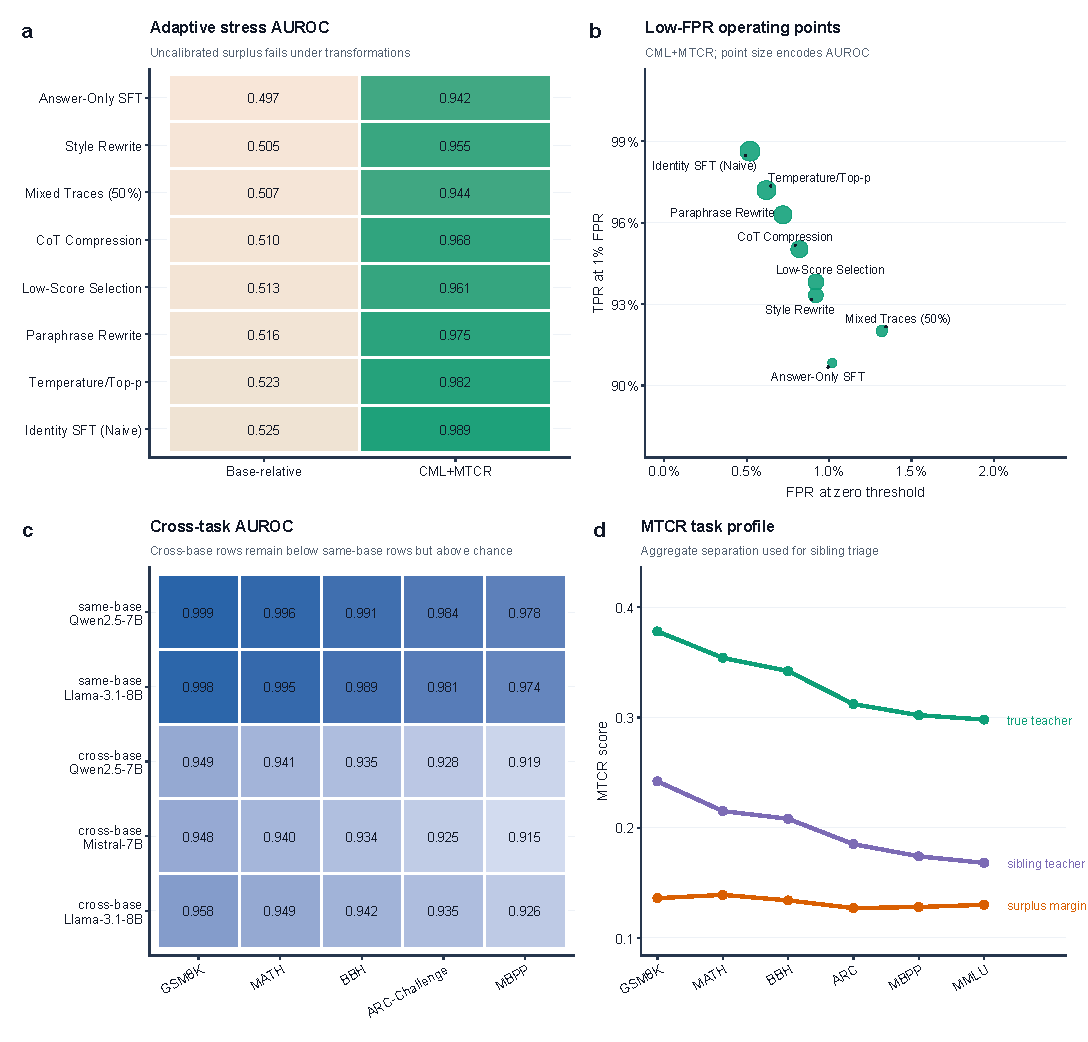
\includegraphics[width=0.98\linewidth]{figures/fig_supp_operating_stress.pdf}
\caption{Supplementary operating-stress diagnostics from the packaged aggregate
source tables. (a) Adaptive trace-transformation AUROC for base-relative surplus and
CML+MTCR. (b) CML+MTCR operating points under the same transformations, plotting
TPR at 1\% FPR against the zero-threshold false-positive rate. (c) Cross-task and
cross-base AUROC matrix; same-base rows remain highest, while cross-base rows remain
above chance under the evaluated tasks. (d) MTCR task-view profile showing separation
between the true teacher, a sibling teacher, and the aggregate surplus margin.}
\label{fig:supp_operating_stress}
\end{figure}

\subsection{Attribution Scaling with Calibration Tasks}
MTCR calibrates candidate log-likelihoods across task views to separate teacher-specific reasoning styles from baseline model capabilities. The main manuscript reports an aggregate sensitivity curve for $M \in \{1, 2, 4, 8, 12, 16\}$ calibration views.
As shown in main-manuscript Fig.~3(b), sibling attribution accuracy scales
monotonically with the number of calibration tasks. At $M=1$ (which corresponds to
standard CML without cross-task calibration), attribution accuracy within the
DeepSeek-R1 sibling family remains low (0.672 for Qwen-32B and 0.658 for Llama-8B).
When $M$ is increased to 16 tasks, accuracy improves to 0.894 and 0.875,
respectively, indicating that diverse cross-task calibration is useful for
fine-grained provenance tracking inside the declared candidate set. Supplementary
Fig.~\ref{fig:supp_operating_stress}(d) gives the complementary task-profile view:
the true-teacher profile remains separated from the sibling-teacher and surplus-margin
profiles across GSM8K, MATH, BBH, ARC, MBPP, and MMLU task views.

\subsection{Evaluation Trace Budget}
To assess the minimum number of suspect model outputs needed to detect distillation descent, we evaluate the detection AUROC as a function of the number of evaluated traces $N \in \{10, 20, 50, 100, 200, 500\}$ sampled from the suspect model.
Main-manuscript Fig.~4(a,b) demonstrates the sample-size requirements. When only 10
traces are evaluated, the high variance in token log-probabilities yields moderate
AUROC scores (0.712 for Qwen and 0.695 for Llama). However, the variance shrinks
rapidly as $N$ increases; the detection AUROC exceeds 0.95 at $N=100$, and converges
near 1.00 at $N=500$ within this evaluated query-budget sweep.

\subsection{Influence of Reasoning Step Depth}
Distillation footprints are primarily encoded in the reasoning style and formatting patterns of the teacher model. We analyze the impact of the suspect model's reasoning chain length by filtering traces based on the minimum number of reasoning steps.
As illustrated in main-manuscript Fig.~4(c), CML performance improves as the
reasoning depth increases. For short derivations (minimum step depth of 2), the
detection AUROC is 0.924 (Qwen) and 0.915 (Llama). For longer, more complex reasoning
chains (step depth $\ge 8$), the AUROC approaches 0.999. This suggests that more
extensive reasoning chains carry denser stylistic and descent-specific markers.

\subsection{Cross-Dataset Operating Sensitivity}
To check whether a detector calibrated on one task can generalize to other domains, we evaluate students distilled on GSM8K using traces drawn from SVAMP, ASDiv, MATH, and ARC-Challenge.
Main-manuscript Fig.~4(d) shows that the distillation footprint remains detectable
across the evaluated reasoning datasets. Even when evaluated on out-of-domain tasks
like MATH (AUROC 0.953) or ARC-Challenge (AUROC 0.912), CML+MTCR distinguishes
distilled students from non-distilled controls in this aggregate evaluation. This is
cross-dataset operating-envelope evidence, not a broad deployment guarantee.
Supplementary Fig.~\ref{fig:supp_operating_stress}(c) extends the same point to the
broader cross-task matrix used in the TIFS stress bundle.

\subsection{Sensitivity to Fine-Tuning Hyperparameters}
Finally, we probe whether the detection signature is an artifact of specific student training parameters. We sweep the teacher-forcing temperature $T \in \{0.2, 0.5, 0.8, 1.0, 1.2\}$ and the student supervised-fine-tuning learning rate $\eta \in \{5\times 10^{-6}, 1\times 10^{-5}, 2\times 10^{-5}, 5\times 10^{-5}\}$.
Across all configurations, the detection AUROC remains consistently high (ranging
from 0.981 to 0.999), indicating that the capability-matched test is not driven by
the particular temperature or learning-rate setting used in the main run.
The compact summary is reported in main-manuscript Fig.~4(e,f).
% END expanded input: sections/appendix.tex


\end{document}
